\documentclass[11pt,a4paper]{article}
\usepackage[margin=23mm]{geometry}
\usepackage{fontspec}
\setmainfont{Palatino Linotype}
\usepackage{amsmath,amssymb,graphicx,booktabs,xcolor,hyperref,fancyhdr}
\graphicspath{{../../pn_junction_2d/figures/}}
\definecolor{ink}{HTML}{182A35}
\definecolor{accent}{HTML}{155D64}
\definecolor{muted}{HTML}{4D626D}
\hypersetup{colorlinks=true,urlcolor=accent,linkcolor=accent,
  pdftitle={2D Silicon PN Junction},
  pdfsubject={Math audit, curvature controls and verification}}
\setlength{\parindent}{0pt}
\setlength{\parskip}{5pt}
\setlength{\headheight}{15pt}
\pagestyle{fancy}
\fancyhf{}
\fancyhead[L]{\small\color{muted} Computational physics}
\fancyhead[R]{\small\color{muted} PN junction simulation}
\fancyfoot[R]{\small\color{muted}\thepage}
\renewcommand{\headrulewidth}{0.3pt}
\newcommand{\um}{\,\mu\mathrm{m}}
\newcommand{\figtext}[1]{{\small\color{muted}#1\par}}

\begin{document}
\thispagestyle{plain}
{\large\color{accent} Computational physics \hfill 25 November 2026\par}
\vspace{5mm}
{\Huge\bfseries\color{ink} 2D silicon PN junction\par}
\vspace{2mm}
{\Large\color{muted} Math audit, curvature controls and verification\par}
\vspace{4mm}

\textbf{Summary.} The drift--diffusion equations, signs and scaling agree
with the implementation. The original amplitude sweep gave a \(2.47\%\)
increase in peak field at \(A=0.40\um\). Holding the doping transition
scale fixed along the local normal instead gives a \(3.33\%\) decrease.
Both trends persist on the refined mesh. This is a controlled comparison
of two doping models for the same device shape.

\textbf{Scope.} The audit covered the Python solver, geometry, configuration,
discrete operators, post-processing, CLI, tests, notebook and writeups at
\href{https://github.com/johntheseegler/pn-junction-sim/tree/7865f004aefdff5889c56161ae058d7ed4d330b7}{commit \texttt{7865f00}}.
The updated local copy retains the original horizontal doping model and
adds a signed-distance model, reference benchmarks, plots and run diagnostics.

\section*{1. Governing equations and discretization}
The model is steady-state and uses cm-based semiconductor units.
Take the p contact on the left, with positive applied voltage \(V\) for
forward bias. Both contacts are ideal and ohmic. The top and bottom walls
have zero normal electric and carrier flux. The simulator assumes
Boltzmann statistics, fully ionized dopants, constant mobility and
permittivity, and midgap Shockley--Read--Hall (SRH) recombination.
\begin{align*}
\nabla^2\psi &=-\frac{q}{\varepsilon}(p-n+N_{\rm net}),\qquad
  \mathbf E=-\nabla\psi,\\
\mathbf J_n &=q\mu_n n\mathbf E+qD_n\nabla n,\qquad
\mathbf J_p=q\mu_p p\mathbf E-qD_p\nabla p,\\
\nabla\cdot\mathbf J_n &=qR,\qquad \nabla\cdot\mathbf J_p=-qR,\qquad
D_{n,p}=\mu_{n,p}V_T,\\
R&=\frac{np-n_i^2}{\tau_p(n+n_i)+\tau_n(p+n_i)},\qquad
V_T=k_{\mathrm B}T/q .
\end{align*}
Set \(C_0=\max(N_A,N_D)\) and \(L_D^2=\varepsilon V_T/(qC_0)\).
Scaling potential by \(V_T\), densities by \(C_0\), and position by \(L_D\)
gives the discrete Poisson residual \(L\tilde\psi-\tilde n+\tilde p+\tilde N\).
With quasi-Fermi potentials fixed, differentiating the Boltzmann factors
gives the interior Jacobian \(L-\operatorname{diag}(\tilde n+\tilde p)\).
The contact residual is prescribed potential subtracted from the
current potential iterate.

For a directed face with \(z=\tilde\psi_b-\tilde\psi_a\),
the Scharfetter--Gummel weights use \(B(z)=z/(e^z-1)\).
The identity \(B(-z)=e^z B(z)\) cancels the electron flux for
\(\tilde n_b=e^z\tilde n_a\) and the hole flux for
\(\tilde p_b=e^{-z}\tilde p_a\). The Gummel iteration couples the
Poisson update to the two continuity solves with lagged SRH coefficients.
Shared face fluxes and half cells at the zero-flux walls give a
conservative finite-volume balance. Integrating \(J_{n,x}+J_{p,x}\)
over \(y\) yields current per out-of-plane depth in A/cm.

\newpage
\section*{2. Planar references and verification}
The neutral Boltzmann contacts have \(p_L-n_L=N_A\),
\(n_R-p_R=N_D\) and \(np=n_i^2\). Combining these equations gives
\[
V_{\rm bi}=V_T\left[
\operatorname{asinh}\!\frac{N_A}{2n_i}+
\operatorname{asinh}\!\frac{N_D}{2n_i}\right].
\]
For \(N_A,N_D\gg n_i\), this reduces to \(V_T\ln(N_A N_D/n_i^2)\).
In the abrupt depletion approximation, the integrated charge implies
\(N_Ax_p=N_Dx_n\). Integrating the triangular field gives
\[
W_d^2=\frac{2\varepsilon}{q}\left(\frac1{N_A}+\frac1{N_D}\right)(V_{\rm bi}-V),
\qquad
\lvert E_{\max}\rvert=\frac{2(V_{\rm bi}-V)}{W_d}.
\]
The classical helper now requires \(V<V_{\rm bi}\). The old helper
subtracted \(2V_T\) by default and returned \texttt{nan} at \(+0.70\) V.
The new symmetric equilibrium reference uses the first integral of
Poisson--Boltzmann for an abrupt step. With \(N=N_A=N_D\) and
the junction at the zero of potential, it gives
\[
\lvert E_{\rm PB}\rvert^2
=\frac{2q}{\varepsilon}
\left[\frac{NV_{\rm bi}}{2}
-V_T\left(\sqrt{N^2+4n_i^2}-2n_i\right)\right].
\]
The mobile-charge term becomes the familiar \(2V_T\) correction to
the full barrier for \(N\gg n_i\). The simulated half-density width
uses crossings at \(p=N_A/2\) and \(n=N_D/2\).

\medskip
\begin{tabular}{@{}p{0.69\linewidth}r@{}}
\toprule
\textbf{Default 300 K planar benchmark} & \textbf{Result}\\
\midrule
Built-in voltage & \(0.714317\) V\\
2D versus four-times-finer 1D solution, maximum potential difference & \(0.332\) mV\\
Simulated half-density width & \(0.4161\um\)\\
Classical abrupt width & \(0.4298\um\)\\
Simulated peak field & \(26.391\) kV/cm\\
Classical abrupt peak field & \(33.238\) kV/cm\\
Abrupt Poisson--Boltzmann peak field & \(32.012\) kV/cm\\
\bottomrule
\end{tabular}

\medskip
The planar grid is \(201\times81\) over \(4\um\times2\um\).
It uses \(N_A=N_D=10^{16}\,\mathrm{cm}^{-3}\),
\(n_i=10^{10}\,\mathrm{cm}^{-3}\) and horizontal tanh scale \(w=0.0625\um\).
The relative permittivity is \(11.7\), the mobilities are
\(\mu_n=1400\) and \(\mu_p=450\,\mathrm{cm}^2/(\mathrm{V\,s})\),
and both SRH lifetimes are \(1\,\mu\mathrm{s}\).
The simulated equilibrium peak field is \(17.6\%\) below the
Poisson--Boltzmann reference. A resolved 1D sweep reducing \(w\)
from \(0.08\um\) to \(0.01\um\) cuts this deficit from \(20.9\%\) to
\(3.3\%\). This checks the expected sharp-junction limit.

For asymmetric doping the zero of the tanh net-doping profile occurs at
the signed coordinate \(d_0=(w/2)\ln(N_A/N_D)\). The curve is the midpoint
of the grading. The asymmetry test checks this zero, the contact neutrality
conditions and the resulting built-in potential.

\newpage
\section*{3. Curvature and the doping transition}
For \(f(y)=L_x/2+A\cos(2\pi y/L_y)\), the maximum interface curvature
is \(\kappa_{\max}=A(2\pi/L_y)^2\). The horizontal tanh uses \(d=x-f(y)\).
Its local normal transition scale is \(w/\sqrt{1+f'(y)^2}\).
At \(A=0.40\um\), it drops from \(0.11\um\)
to \(0.0685\um\) on the steepest flank. The new profile uses the closest-point
distance to the cosine, positive on the n side, with the same nominal
\(w=0.11\um\). Both devices use the same \(-2\) V bias and \(2\um\) wavelength.

\medskip
\begin{tabular}{@{}rrrr@{}}
\toprule
\(A\) (\(\mu\)m) & \(\kappa_{\max}\) (\(\mu\mathrm{m}^{-1}\)) &
\textbf{Horizontal (kV/cm)} & \textbf{Signed distance (kV/cm)}\\
\midrule
0.00 & 0.000 & 54.154 & 54.154\\
0.10 & 0.987 & 54.300 & 53.977\\
0.25 & 2.467 & 54.745 & 53.105\\
0.40 & 3.948 & 55.492 & 52.351\\
\midrule
0.00, refined & 0.000 & 54.193 & 54.193\\
0.40, refined & 3.948 & 55.534 & 52.377\\
\bottomrule
\end{tabular}

\begin{center}
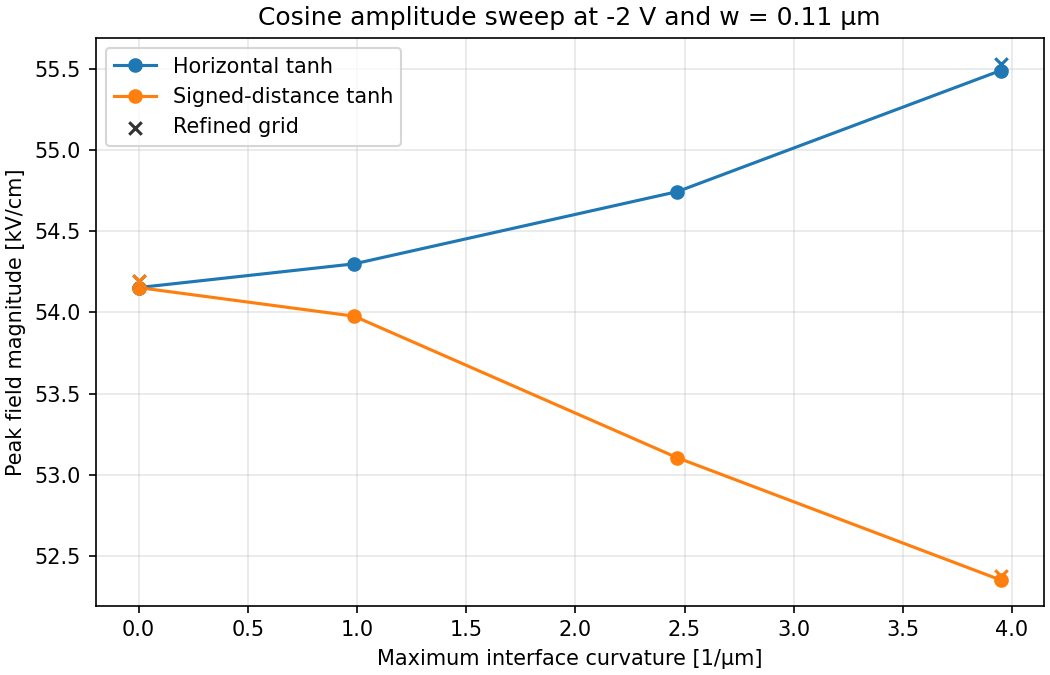
\includegraphics[width=0.83\linewidth]{emax_vs_curvature.png}
\end{center}
\figtext{\textbf{Figure 1.} Peak field magnitude across the four tested amplitudes.
The crosses repeat the planar and largest amplitude cases on a
\(401\times161\) grid, with the physical transition scale held fixed.}

Refining the mesh changes each endpoint peak by less than \(0.08\%\).
Relative to its planar value, the largest-amplitude profile changes
by \(+2.47\%\) (horizontal) and \(-3.35\%\) (signed distance) on the refined mesh.
The sweep varies slope and curvature together. The difference between
the two curves quantifies sensitivity to how the doping follows the geometry.

\newpage
\section*{4. Where the peak field occurs}
\begin{center}
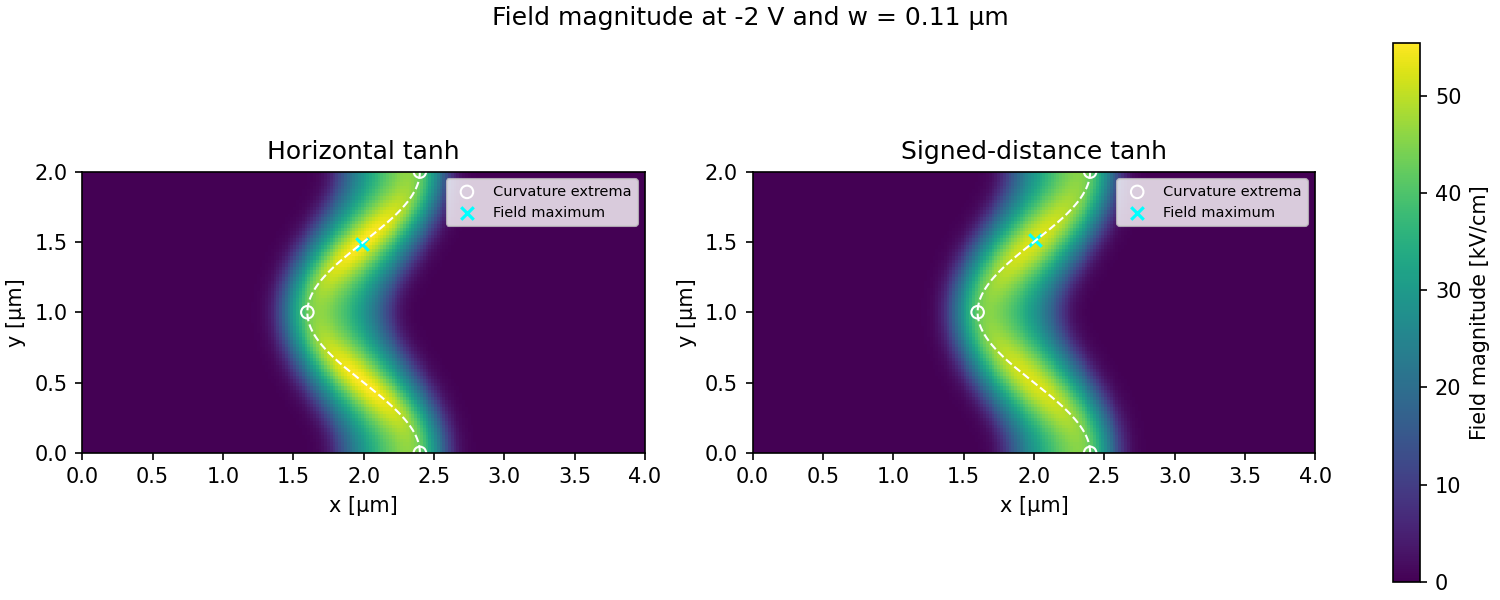
\includegraphics[width=\linewidth]{curvature_field_comparison.png}
\end{center}
\figtext{\textbf{Figure 2.} Field magnitude for \(A=0.40\um\) on a shared color
scale. The dashed line is the junction curve. Circles mark the local
curvature maxima and crosses mark one of the sampled field maxima.}

Both profiles reach their peak near the steep flanks. In the original
profile, the interface curvature at the sampled peak's \(y\)-coordinate is
about \(0.04\,\mu\mathrm{m}^{-1}\) on the base grid. It reaches
\(3.95\,\mu\mathrm{m}^{-1}\) at the tips. Reflection symmetry gives two
equivalent flanks, so the mesh and round-off can change which peak is reported.

\begin{center}
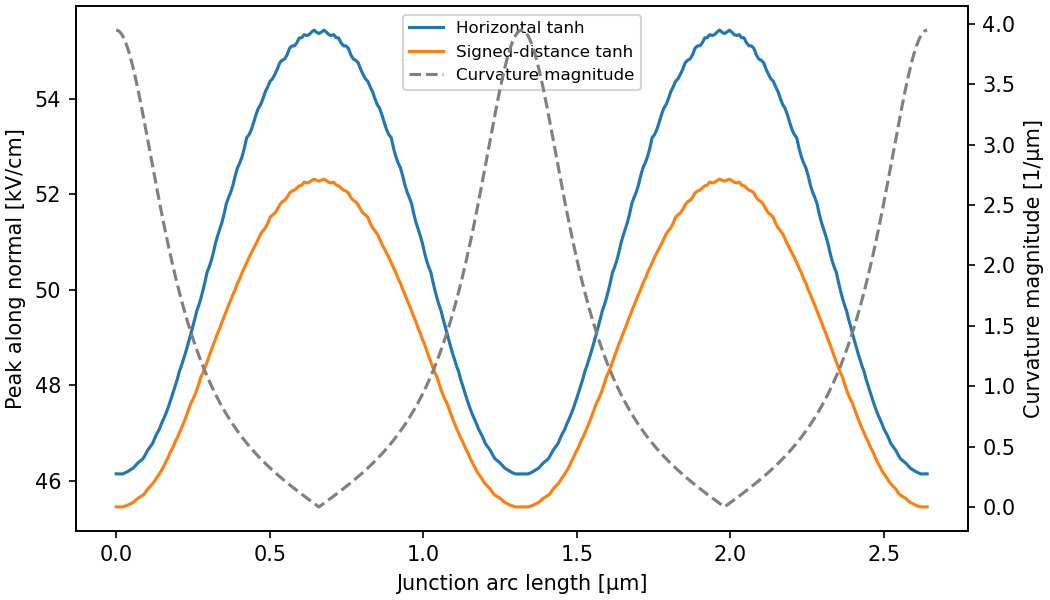
\includegraphics[width=0.86\linewidth]{curvature_normal_profiles.png}
\end{center}
\figtext{\textbf{Figure 3.} Peak magnitude along junction-normal segments plotted
against interface arc length. Each segment spans one classical depletion
width on either side. The dashed gray line shows the curvature magnitude
on the right axis. This resolves the field maxima relative to the tips.}

\newpage
\section*{5. Bias sweep and diagnostics}
The planar sweep spans \(-3.0\) to \(+0.65\) V over 29 bias points.
The forward slope over \(0.25\) to \(0.55\) V gives an ideality factor
of \(1.008\). A finite-base, low-injection diffusion estimate at
\(+0.45\) V gives \(2.976\times10^{-6}\) A/cm, compared with
\(2.981\times10^{-6}\) A/cm numerically. The estimate uses the neutral
region lengths \(\ell\) from the classical depletion edges to the contacts.
For each minority carrier, solving the diffusion--recombination equation
with excess density zero at the contact gives an edge contribution
\(q(D/L)\coth(\ell/L)\Delta c\), where \(L=\sqrt{D\tau}\) and
\(\Delta c\) follows the low-injection junction law.

\begin{center}
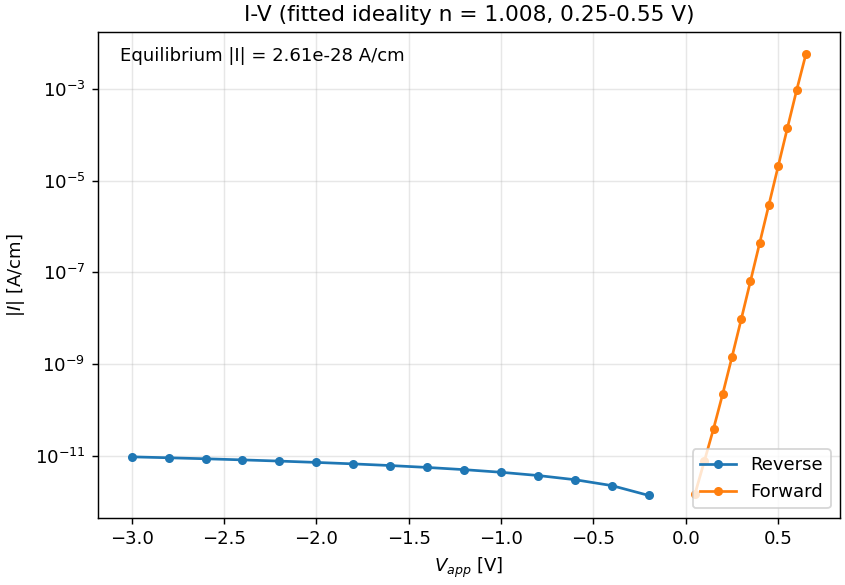
\includegraphics[width=0.49\linewidth]{iv_planar.png}\hfill
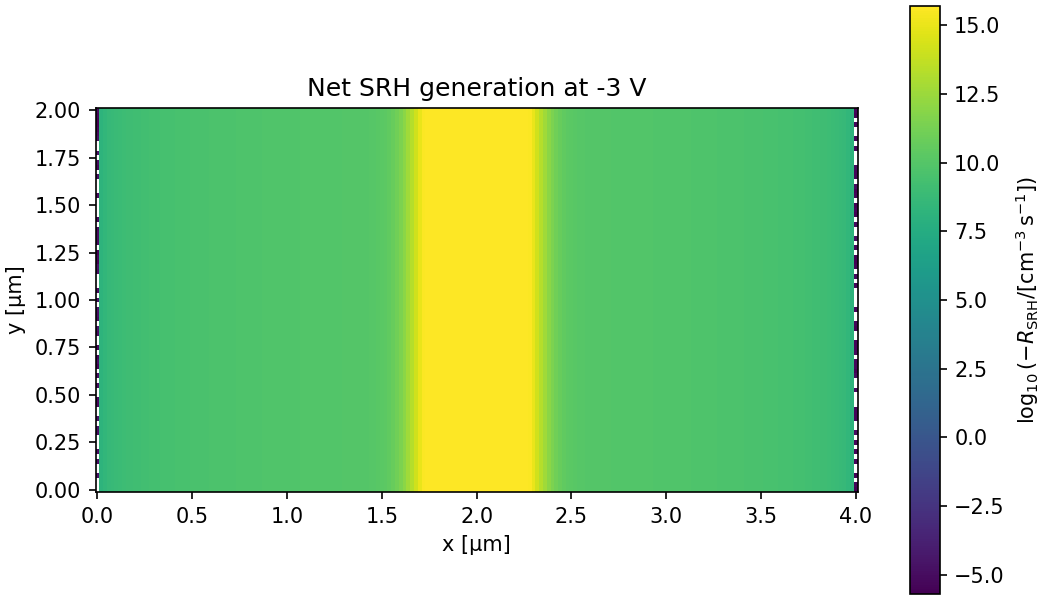
\includegraphics[width=0.49\linewidth]{srh_generation_reverse.png}
\end{center}
\figtext{\textbf{Figure 4.} Forward and reverse branches of the planar I--V sweep
and positive net SRH generation at \(-3\) V. The reverse generation
is concentrated around the depletion region. The equilibrium current is
shown as an annotation to preserve the dynamic range of the I--V axes.}

The maximum relative column-current deviation over the nonzero planar
biases is \(9.7\times10^{-7}\). At equilibrium the mean is
\(2.61\times10^{-28}\) A/cm and the absolute deviation is
\(9.07\times10^{-29}\) A/cm. Reporting the relative value there would
inflate the apparent error to about \(35\%\).

\texttt{iv\_diagnostics.csv} exports both contact currents signed in \(+x\),
the mean, absolute and relative deviations, scaled Poisson residual and both
continuity residuals in \(\mathrm{cm}^{-3}\,\mathrm{s}^{-1}\). It also records
the peak field and coordinates, Gummel iterations and round-off status.
The relative deviation is undefined at or below \(10^{-20}\) A/cm.
\texttt{curvature\_diagnostics.csv} records the profile, mesh, amplitude,
bias, transition scale, maximum curvature, peak field, position and current.

\section*{6. Reproduction and scope}
Install the requirements and run both studies and the regression suite
from the local project root.
{\small\begin{verbatim}
python -m pip install -r pn_junction_2d/requirements.txt
python pn_junction_2d/main.py
python -m pytest -q pn_junction_2d/tests
\end{verbatim}}
All 24 tests passed. The notebook imports the same study functions.
The local copy includes a GitHub Actions workflow for Python 3.12,
a Quick Start and ignore rules for interpreter and notebook caches.

The results verify the implemented steady-state model against analytic
limits, grid refinement and numerical balances. The simulated current
and field magnitudes still need experimental calibration for a specific device.

\figtext{\textbf{References.}
\href{https://ocw.mit.edu/courses/6-012-microelectronic-devices-and-circuits-fall-2009/c053714447998e522f02db0776987091_MIT6_012F09_lec04.pdf}{MIT OCW, \emph{p--n Junctions: Electrostatics}}.
\href{https://homepages.iitb.ac.in/~alsangle/MM765_Lecture_8.html}{IIT Bombay, \emph{Semiconductor Devices, Lecture 8}}.
\href{https://sesame.readthedocs.io/en/latest/physics/}{NIST Sesame, \emph{Analytical Model and Numerical Implementation}}.}
\end{document}
